\section{SYSTEM ARCHITECTURE}
The global architecture for the system is presented in \autoref{fig:finalArchitecture}.

\begin{figure}[H]
    \centering
    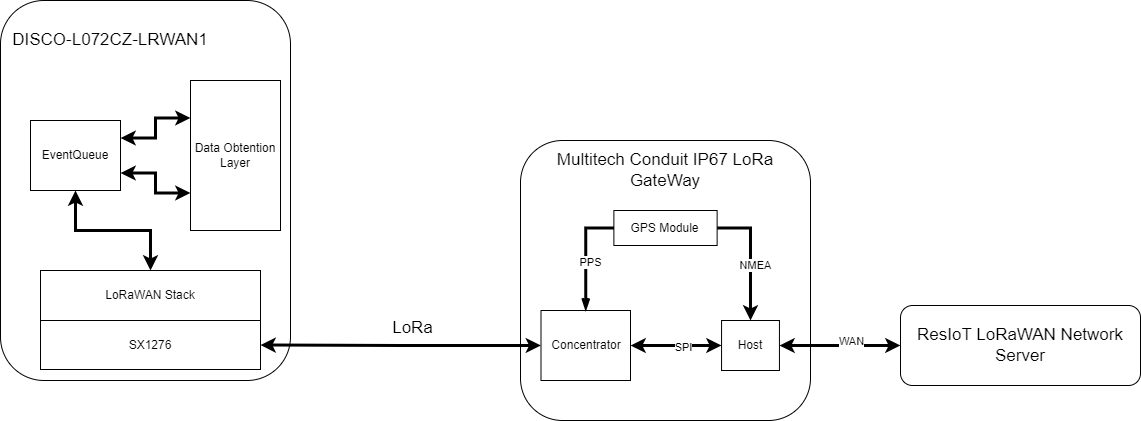
\includegraphics[width=1\textwidth]{images/3/Modules.drawio.png}
    \caption{Final system architecture}
    \label{fig:finalArchitecture}
\end{figure}

\subsection{\acrshort{lorawan} module}

To communicate the data obtention platform, the board\cite{DISCOL072CZLRWAN1Mbeda} includes the \texttt{SX1276}\cite{SX1276} \acrfullr{spi} module in the packaging.

As the radio communication subsystem of \acrshort{lorawan} is proprietary, the module is developed by Semtech.

This module implements a LoRa Modem, with some specific characteristics that are going to be transparent for the development of this project but are important to understand:
\begin{itemize}
    \item Sensibility down to \texttt{-148 dBm}.
    \item An integrated \texttt{+20 dBm} power amplifier.
    \item A bitrate up to \texttt{300 kbps}.
    \item A low RX current of \texttt{9.9 mA}.
    \item Apart from the LoRa modulation, it also supports \acrfullr{fsk}, \acrfullr{gfsk}, \acrfullr{msk} and \acrfullr{gmsk}.
    \item Compatibility with another wireless system, Sigfox.
\end{itemize}

All this information was obtained from the reference datasheet.

Finally, the high level protocol stack is provided by Mbed-OS and by examples.
\clearpage
\subsection{Gateway}

To intercommunicate the different protocols stacks of the system, a Gateway is used. The gateway is shown in \autoref{fig:gateway}.

\begin{figure}[H]
    \centering
    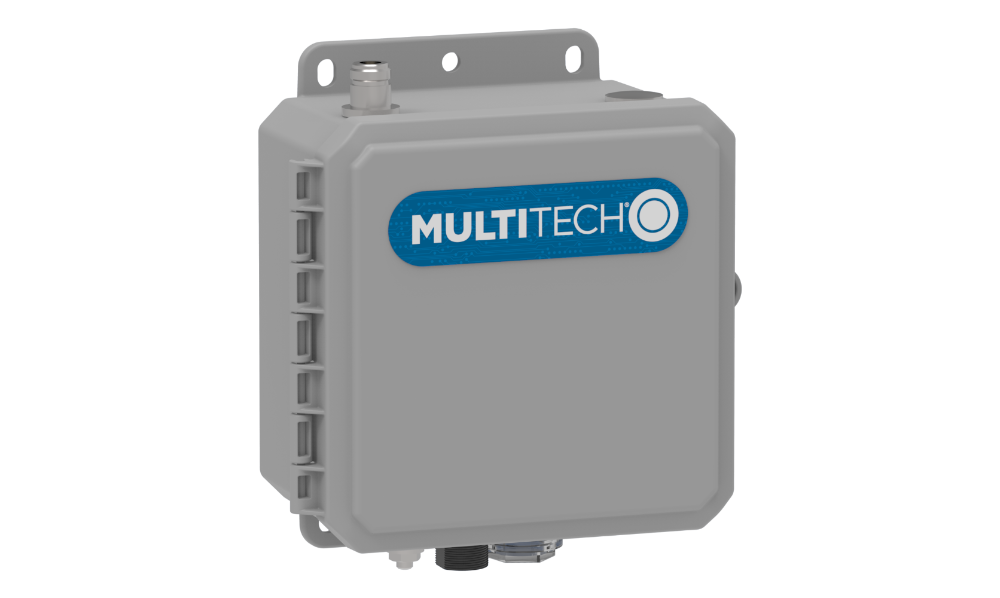
\includegraphics[width=0.7\textwidth]{images/3/multitechip67200.png}
    \caption{Multitech conduit 210/220 series}
    \label{fig:gateway}
\end{figure}

The gateway is powered by an \texttt{32bit ARM9} processor. It's composed by 3 main parts:
\begin{itemize}
    \item A concentrator that focuses on obtaining data from the \acrshort{lorawan} signals. In this case, it uses the Europe frequency band, \texttt{868 MHz}.
    \item A host that processes the \acrfullr{rf} messages and communicates with the network serve, in this case, the ResIoT instance. The interface used for this communication is an Ethernet \texttt{10/100 Base T}.
    \item Finally, a \acrfullr{gnss} module that supports GPS, Galileo or QZSS systems.
\end{itemize}

Some extra features of the gateway that are not used for this project are:
\begin{itemize}
    \item Wi-Fi communication capabilities.
    \item BT Classic and \acrfullr{ble}.
    \item Backhaul can also be connected through cellular networks.
\end{itemize} 

All this information was taken from the datasheet of the gateway\cite{MultiTechConduitIP67}.

The gateway is located in the roof of the Building 8.

